% Document class `report-template` accepts either project-plan or final-report option in [].
\documentclass[project-plan]{report-template}

% Packages I use in my report.
\usepackage{graphicx}
\usepackage{amsmath}
\usepackage{blindtext}

% Directory where I saved my figures.
\graphicspath{{./figures/}}

% Metadata used for the title page - please modify.
\university{Imperial College London}
\department{Department of Earth Science and Engineering}
\course{MSc in Environmental Data Science and Machine Learning}
\title{Building a route optimisation system that takes elevation into consideration}
\author{Jinsong Dong}
\email{jinsong.dong22@imperial.ac.uk}
\githubusername{edsml-jd622}
\supervisors{Sesinam Dagadu\\
             Dr. Yves Plancherel}
\repository{https://github.com/ese-msc-2022/irp-jd622}

\begin{document}

\maketitlepage  % generate title page

% Abstract
\section* {Abstract}
The Traveling Salesman Problem (TSP) is a route optimization problem that aims to minimize the path given a series of locations.
 Extensions of the route optimization problem can involve optimizing for minimum fuel/battery consumption, emissions, traveling time, and more. 
 This project is an external project from SnooCode, with the goal of designing a route optimization system for a delivery company that utilizes battery bikes, 
 taking into consideration the elevation.\\

The project is divided into two parts: data processing and model development, 
as well as route optimization algorithms. 
This subproject focuses on the first part. 
The main objectives of this subproject are as follows: 
developing a 3D road network for Accra by combining the 2D road network data with raster elevation data, 
creating an electric bike model using Python to calculate battery consumption and traveling time, 
combining the 3D road network and the e-bike model to create a comprehensive model.\\

Once the model is developed, 
it can be integrated with route optimization algorithms to determine the best route for the delivery company based on different optimization goals 
such as shortest path, minimum battery consumption, traveling time, and more.\\

This project plan provides details about the project, 
including the progress made to date and the future plans.

% Introduction section
\section {Introduction}
\subsection {Literature Review}
The route optimisation problem in this project is a kind of Travel Salesman Problem(TSP) \cite{lawler1985travelling}, 
which means given a list of cities and distances between each pair of cities, what is the shortest possible
route that visits each city exactly once and returns to the origin city \cite{TSP_wiki}. 
TSP is a classic NP-hard problem, means it can not be solved in polynomial time.
One example of a solution of a TSP is shown in Fig.~ \ref{fig:solution_of_TSP}.
In this example, there are 35 locations in total, and the shortest way between these locations are drawn in the line.
There are $35!$ possible combination of the route totally, the 'brute-force solution' will take a very long time to get the results.\\
\begin{figure}
    \begin{center}
        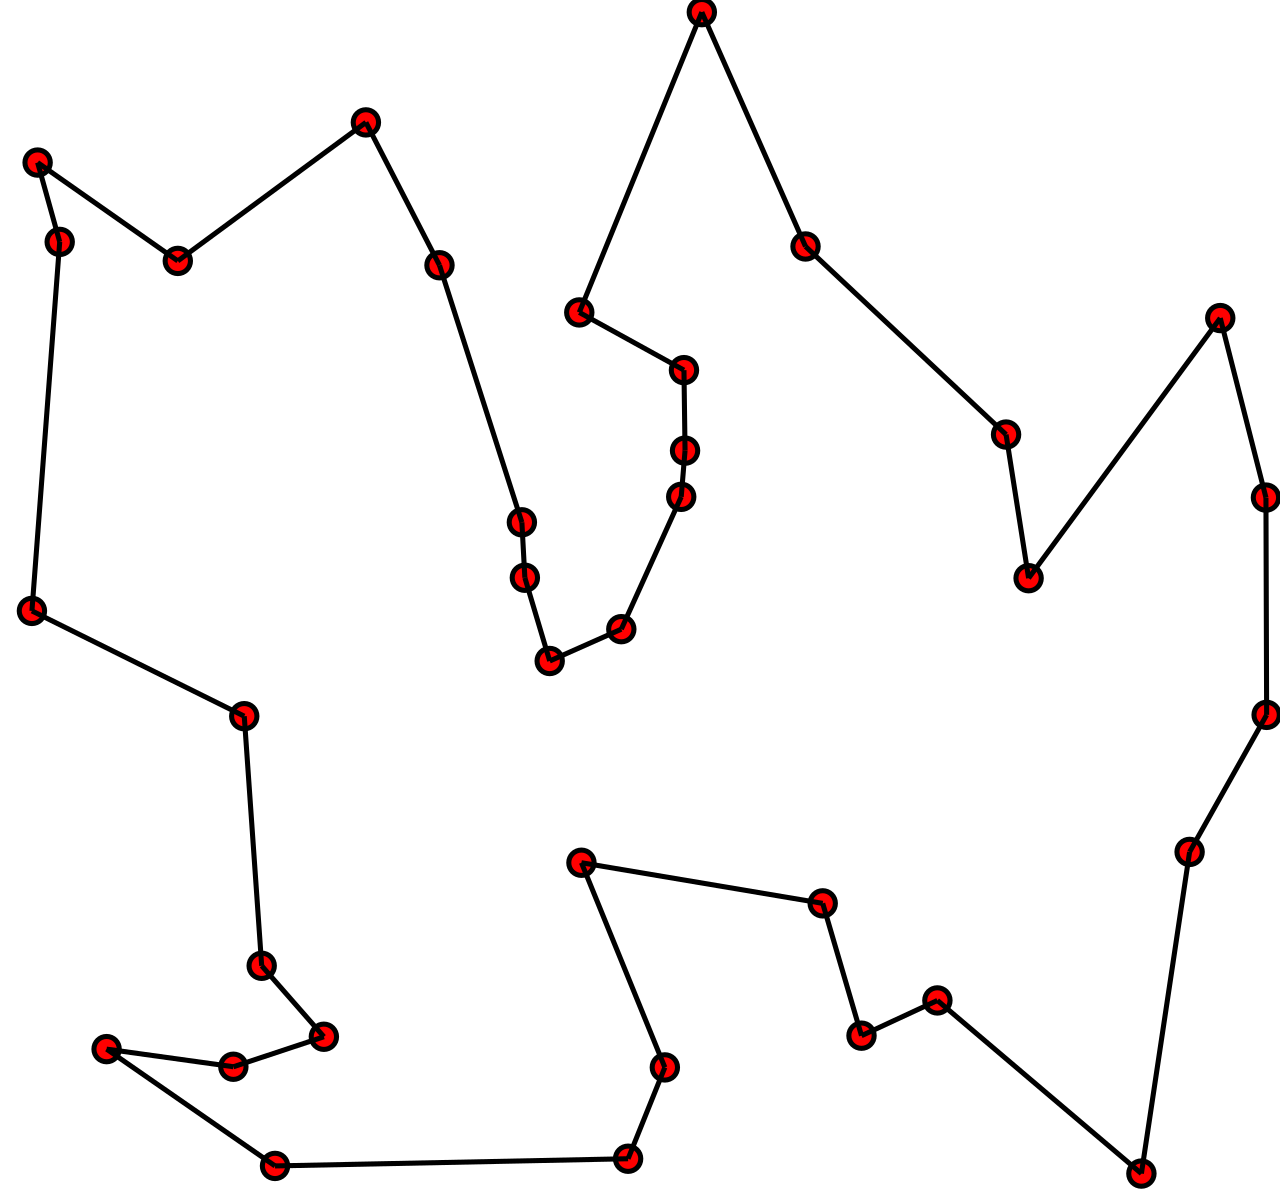
\includegraphics[width=0.2\textwidth]{solution_of_a_TSP.png}
    \end{center}
    \caption{\label{fig:solution_of_TSP} A solution example for TSP.}
\end{figure}

Algorithms to reduce the calculation time is essential. Many heuristic algorithms have been utilized in solving TSP\cite{TSP_review},
for example: ant algorithm, greedy method, simulated annealing, tabu search and genetic algorithm \cite{genetic_on_TSP}. 
Genetic algorithm randomly samples values of the changing cells between lower and upper bounds to generate
a set of combination of possible route, and choose the best one.
Genetic algorithm can give a near to optimal solution in a relatively short time, but we cannot know how near it can be to the best route.
Ant Colony Optimization algorithm(ACO) is one of the metaheuristic methods for solving TSP, 
it works like observation of real ants, and upon finding food return to their colony while laying down pheromone trails\cite{ACO_on_TSP}. 
The ACO can also get a near-optimal solutions to the traveling salesman problem, it's able to find the global optimum in a finite time.
Some improved ACO algorithms have also been proposed like Parallel implementation of ant colony optimization \cite{para_ACO}. 
Christofides algorithm\cite{VANBEVERN2020118} utilizes Minimum spanning tree(MST) to get the approximation solution of traveling salesman problem, 
which guarantees its solutions will be within a factor of 3/2 of the optimal solution length.
Christofides algorithm has the limitation that it can only be applied on the instances where the distances form a metric space (they are symmetric and obey the triangle inequality) \cite{christofides_inbook}.
Simulated annealing(SA) algorithm is a kind of greedy algorithms. It uses randomness as part of its search for the best solution, so it is a stochastic global search algorithm.
Simulated annealing algorithm is good at jumping out of the local minimum\cite{improved_SA}.\\

The algorithms mentioned above are mainly used on optimizing the shortest way to go, in addition to these, the work by Dijkstra based on the graph-theory also focus on the shortest path.
Routing optimization has been extended into the domain of logistic, respective extensions are called VRP\cite{BRAEKERS2016300}, VRP not only optimize the distance between two single points,
but also optimize the distances between a series points under different criterion and restrictions. 
Some research extended VRP to green logistic, they optimize the fuel consumption and emissions\cite{green_vehicle}.
Marc Schröder and Pedro Cabral\cite{article} build a model to estimate the $CO_2$ emissions for road freight transportation and found eco-friendly route can yield up to 20\% emissions reduction.
Jiquan Wang\cite{battery_predict} develop an energy consumption prediction algorithm to make route optimisation for electric vehicles.\\

These researches about the extensions of route optimisation did case studies on different areas like Korea and Portugal, they focused on freight trucks and electric vehicles.
However, no one has done route optimisation for minimize battery consumption research for electric bikes, and no case study in Ghana yet. 
This project will focus on the eco-friendly route optimization system on electric bikes, and make several case studies in Accra Ghana.

\subsection {Problem Description}
Snoocode Corporation has designed a route optimization system that works offline on a smartphone and provides 
results 42000 times faster than the conventional method. However, this method only consider a 2D map.
The next step for Snoocode is developing and incorporate an algorithm that considers land elevation. 
In this method, I need to optimize the route in a 3D map, as elevation is a very important factor for 
electric bikes and bicycles. \\

To be more specific about the function of the route optimisation system, suppose we have 20 locations to
give delivery to, we need to find the shortest way to go so that we can deliver to every location. 
But in this case, a very important thing is to consider altitude, 
because the transportation in this project is electric bike, altitude can have a significant impact on the battery consuming.
Moreover, the route optimization system should not only be able to optimize the length of the way, but also the battery consuming, time consuming.\\

In this project, we divide the problem into two parts: One part is data processing, which is my main objective, the other one part is building route optimization algorithm, which will be done by Rutvji Kulkarni.
These two parts will be carried on simultaneously, the algorithm part will use the traditional distance to make route optimization temprally.
After two parts are both finished, they will be pulled together to make the final case study.\\

For my main part which is data processing, I need to gather the 2D road data and the raster elevation data for Accra region in Ghana, and combine them together into a 3D-road network.
Then I should build an electric bike model which is used to calculate the battery consuming and traveling time.
After that I should calculate some attributes including average velocity on each road segment, road slope and add them into the 3D-road network.
Finally, all models I made should be integrated with the route optimization algorithm from Rutvji and make specific study case.

\subsection {Objectives}
The project will be split into two parts. 


As the data processing part is my main objective, this part will be described with more detail,
and the other part done by Rutvji will be described in short and with label. 
The project has four objectives below:
\begin{itemize}
    \item Data collection and pre-processing: gather data for Accra region in Ghana that in
          relevant to the delivery region mentioned before, cut them in the size appropriately and extract the roads needed in the project. 
    \item 3D-road network construction: combine the 2D-road data and the raster elevation data into 3D-road data.
          After construction, calculate several attributes and add them into every road segment in the 3D-road network, including: average velocity on the road, road slope, 3D-lengths.
          These attributes are essential for calculating battery consuming and time-consuming on the road.
    \item Electric bike model development in Python: develop an electric vehicle model
          using the data provided by SnooCode
          use this model to calculate the time travelled, battery consuming for the delivery.
          This model can provide the optimization objective function for the route optimization part.
    \item (Rutvji's part)Algorithm development in Python: develop route optimization heuristic algorithms optimising on simple distance, benchmark these methods and determine the most optimal ones. 
    \item Combination of the two parts: integrate the 3D-road network, the electric vehicle model and the route optimisation algorithms together, 
          so that the program can optimize the route with metrics selected by users, including: battery consuming, time consuming, the shortest 3D-lengths.
\end{itemize}

\section {Progress to Date}
\begin{itemize}
    \item Had online-meeting with all the stakeholders of this project, defined the problem we need to solve precisely.
    \item Come up with clear objectives that need to be implemented in details.
    \item Learned algorithms including: Christofides algorithms, Simulated Annealing and Dijkstra's algorithm.
    \item Collected 2D road data of Ghana region, as shown in Fig.~ \ref{fig:ghana_road}. 
    \item Collected elevation data of Ghana region, as shown in Fig.~ \ref{fig:ghana_elevation}.
\end{itemize}

\begin{figure*}[htbp]
    \centering
    \begin{minipage}[t]{0.48\textwidth}
    \centering
    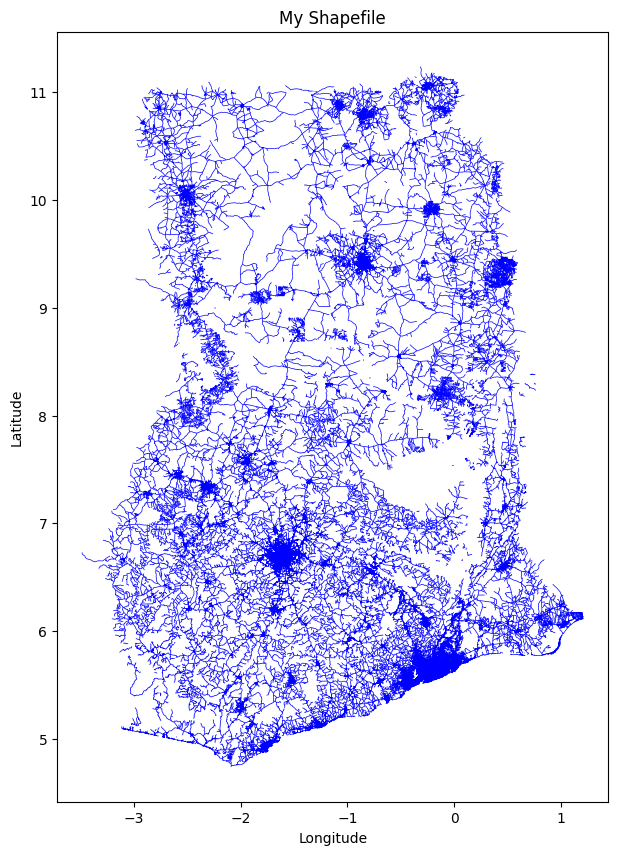
\includegraphics[width=7cm]{ghana_road.png}
    \caption{\label{fig:ghana_road} The 2D-road network of Ghana}
    \end{minipage}
    \begin{minipage}[t]{0.48\textwidth}
    \centering
    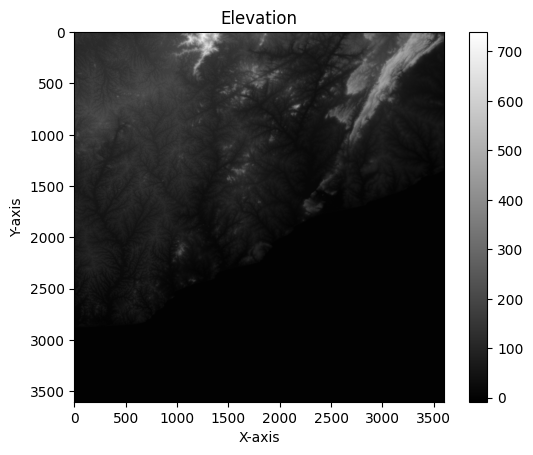
\includegraphics[width=7cm]{ghana_elevation.png}
    \caption{\label{fig:ghana_elevation} The elevation of the region near Accra}
    \end{minipage}
\end{figure*}

\section {Future Plan}
\begin{itemize}
    \item 16/June - 23/June: Integrate 2D road and raster elevation data into 3D-road network.
    \item 24/July - 7/July Implement the electric vehicle model based on the data provided by SnooCode.
    \item 8/July - 24/July: Calculate average speed, road slope, 3D-lengths on each road segment and assign these attributes to the 3D-road network model.
    \item 25/July - 7/August: Make the electric vehicle model.
    \item 8/August - 15/August: Integrate 3D-road model, electric vehicle model and route optimisation algorithm together.
    \item 16/August - 1/September: Tests for all functions, final report.
\end{itemize}

If there is time after implementing obejectives above, the next step is to write a machine learning model or deep learning model
to improve the result of the system. \\

Reinforcement model is a consideration of priority, as it may be hard to get the training dataset.
To train the reinforcement model in this project, I need to build a reinforcement learning agent that can
interact with the environment and learns to choose the optimal order of city visits. 
The agents can select the next city it visits based on the current state(the current city it's in), 
and finally evaluates and optimizes the selection based on the reward signals(the path length/time consuming/battery consuming).


% References
\bibliographystyle{unsrt}
\bibliography{references}  % BibTeX references are saved in references.bib

\end{document}          
